\documentclass[tikz]{standalone}
\usepackage{pgfplots}
\pgfplotsset{compat=1.18}
\definecolor{utnblue}{RGB}{0, 102, 204}

\begin{document}
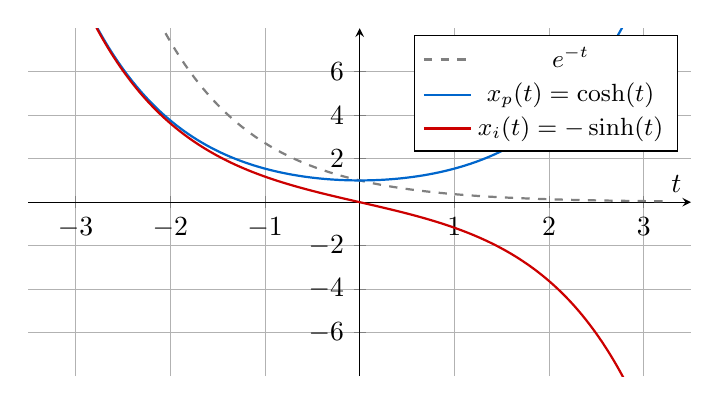
\begin{tikzpicture}
    \begin{axis}[
        width=10cm, height=6cm,
        axis lines=middle,
        xmin=-3.5, xmax=3.5, ymin=-8, ymax=8,
        xlabel={$t$}, ylabel={},
        grid=both,
        grid style={line width=.1pt, draw=gray!40},
        major grid style={line width=.2pt, draw=gray!60},
        xtick={-3,-2,-1,0,1,2,3},
        ytick={-6,-4,-2,0,2,4,6},
        samples=200,
        domain=-3.2:3.2,
        legend style={at={(0.98,0.98)}, anchor=north east, font=\small},
        every axis plot/.append style={thick},
    ]
    % Signal original
    \addplot[gray, dashed] {exp(-x)};
    \addlegendentry{$e^{-t}$}
    % Componente par = cosh(t)
    \addplot[utnblue] {cosh(x)};
    \addlegendentry{$x_p(t) = \cosh(t)$}
    % Componente impar = -sinh(t)
    \addplot[red!80!black] {-sinh(x)};
    \addlegendentry{$x_i(t) = -\sinh(t)$}
    \end{axis}
\end{tikzpicture}
\end{document}
